\documentclass[tikz,border=10pt]{standalone}
\usepackage{tikz}
\usetikzlibrary{positioning,shapes.geometric,arrows.meta,calc}
\usepackage{amsmath}

\begin{document}
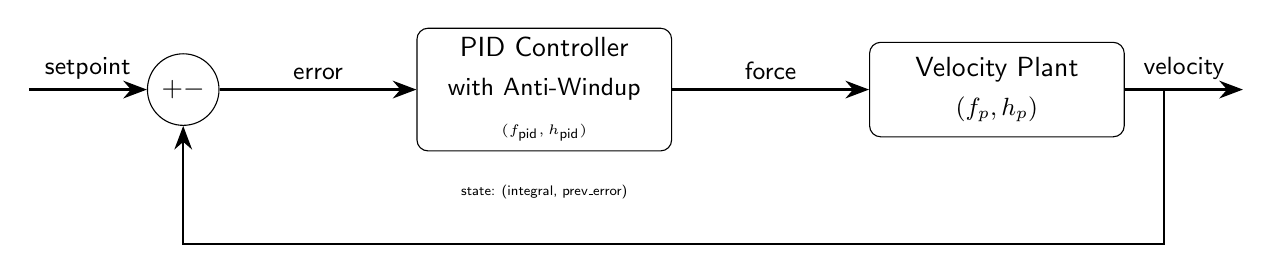
\begin{tikzpicture}[
    node distance=2.5cm,
    block/.style={rectangle, draw, fill=white, text width=3cm, text centered, rounded corners, minimum height=1.2cm, font=\sffamily},
    sum/.style={circle, draw, fill=white, minimum size=0.8cm, font=\sffamily},
    arrow/.style={-{Stealth[length=3mm]}, thick},
    signal/.style={font=\small\sffamily}
]

% Blocks
\node[sum] (sum) {$+$\\[-4pt]$-$};
\node[block, right=of sum] (pid) {PID Controller\\[2pt]{\small with Anti-Windup}\\[2pt]{\tiny $(f_{\text{pid}}, h_{\text{pid}})$}};
\node[block, right=of pid] (plant) {Velocity Plant\\[2pt]{\small $(f_p, h_p)$}};

% Input/Output
\coordinate[left=1.5cm of sum] (input);
\coordinate[right=1.5cm of plant] (output);
\coordinate[below=1.5cm of sum] (feedback_point);

% Forward path
\draw[arrow] (input) -- node[above, signal] {setpoint} (sum);
\draw[arrow] (sum) -- node[above, signal] {error} (pid);
\draw[arrow] (pid) -- node[above, signal] {force} (plant);
\draw[arrow] (plant) -- node[above, signal] {velocity} (output);

% Feedback path
\draw[arrow] ($(plant.east)+(0.5,0)$) |- (feedback_point) -| (sum.south);

% Add state labels
\node[below=0.3cm of pid, signal, align=center] {\tiny state: (integral, prev\_error)};

\end{tikzpicture}
\end{document}
